\documentclass[utf8]{ctexart}
\usepackage{amsmath,mathrsfs,amsfonts,mathtools}%引入数学宏
\usepackage{geometry}%引入编排宏
\usepackage{tikz}%引入画图宏
\usepackage{graphics}%引入排图宏
\usepackage{amssymb}%引入符号库
\usepackage{chemfig}
     
\geometry{a4paper,centering,scale=.85}%A4纸,版心居中,长宽占比0.85

\begin{document}

\zihao{5}
\linespread{2}

\section*{\heiti 初等数学基础知识①———不等式 }

简介:

该篇为复习初等数学的部分内容,其余部分内容参合到高等数学的知识部分里去

一、不等式

不等式在高等数学中十分常用

1、不等式的性质

\begin{align}
    a>b&\Leftrightarrow b<a\\
    a>b,b>c&\Leftrightarrow a>c\\
    a>b&\Leftrightarrow a+c>b+c\\
    a>b,c>0(c<0)&\Leftrightarrow ac>bc(ac<bc)\\
    a>b,c>d&\Leftrightarrow a+c>b+d\\
    a>b>0,c>d>0&\Leftrightarrow ac>bd\\
    a>b>0&\Leftrightarrow a^{n}>b^{n}
\end{align}

2、基本不等式链

\begin{align}
    \displaystyle\sqrt{\frac{\displaystyle\sum^{n}_{i=1}x_{i}^{2}}{n}}\geqslant\frac{\displaystyle\sum^{n}_{i=1}x_{i}}{n}\geqslant \sqrt[\uproot{16}n]{\displaystyle\prod ^{n}_{i=1}x_{i}} \geqslant \frac{n}{\displaystyle\sum^{n}_{i=1}\frac{1}{x_{i}}}
\end{align}

$\text{当且仅当}x_{1}=x_{2}\cdots =x_{n}\text{等号成立}$

3、特殊的不等式

柯西不等式

\begin{align}
    &\displaystyle (x_{1}^{2}+x_{2}^{2}+\ldots +x_{n}^{2})(y_{1}^{2}+y_{2}^{2}+\ldots +y_{n}^{2})\geqslant (x_{1}y_{1}+x_{2}y_{2}+\ldots x_{n}y_{n})
\end{align}

当且仅当$x_{i}(i=1,2,\ldots ,n)=0$或$y_{i}(i=1,2,\ldots ,n)=0$时或$x_{i}=\lambda y_{i}(i=1,2,\ldots ,n)$时等式成立

$(\text{两元形式:当}x_{1}y_{2}=x_{2}y_{1}\text{时等号成立})$

\newpage

\section{\heiti 函数与极限}

\subsection{\heiti 映射}

一、映射

1.映射的概念及其性质

定义1:设$X,Y$是两个非空集合,如果$\exists $一个法则$f$,使得$\forall x\in X$按法则$f$,$\exists $唯一确定的元素$y\in Y$与之对应,那么称$f$为从$X$到$Y$的映射,记作$f:X\to Y$.

其中$y$称为元素$x$(在映射$f$)下的像,并记作$f(x)$,即$y=f(x)$;元素$x$称为元素$y$(在映射$f$下)的一个原像;

集合$X$称为映射$f$的定义域,记作$D_f$,即$D_f=X$;

$X$中所有元素的像组成的集合称为映射$f$的值域,记作$R_f$或$f(X)$,即$R_f=f(X)=\{ f(x)| x\in X\}$.

要注意的是

$(1)$映射三要素:$D_f=X$,$R_f\displaystyle\subseteq Y$,$f$.三要素缺一不可

$(2)$元素$x$的像是唯一的,$y$的原像不一定是唯一的.

若$R_f=Y$,则映射$f$为满射;若$\forall x\in X$有一一对应的像$y\in R_f\subset  Y$,则称映射$f$为单射;若映射$f$即是满射又是单射则称映射$f$为一一映射$(\text{或满射})$

2、逆映射与复合映射

设$f:X \to Y$单射,由定义可得:对$\forall y\in R_f$,有唯一的$x\in X$,适合$f(x)=y$,于是定义一个从$R_f$到$X$的一个新映射$g:R_f\to X$,对$\forall y\in R_f$,规定$g(y)=x$,这个$x$满足$f(x)=y$.这个映射$g$称为$f$的逆映射,记作$f^{-1}$其定义域为$D_{f^{-1}}=R_f$,值域为$R_{f^{-1}}=X$

设有两个映射$g:X\to Y_1\ \ f:Y_2\to Z$,其中$Y_1\subseteq Y_2$,则由映射$g$和$f$可以定义一个从$X$到$Z$的一个对应法则,确定一个从$X$到$Z$的一个映射,这个映射称为由映射$g$和$f$构成的复合映射,记作$f\circ g$,即$f\circ g :X\to Z, \ \ \ (f\circ g)(x)=f\left[g(x)\right] ,\ x\in X$

由复合映射的定义可知:(1)满足条件$R_g\subseteq D_f$;(2)复合映射具有顺序性;(3)$f\circ g$有意义但是$ g\circ f$不一定有,即使有也不一定相等.

\subsection{\heiti 函数}

1、函数的概念

定义2:设数集$D\subseteq  \mathbf{R} $,则称映射$f:D\to  \mathbf{R} $为定义在$D$上的函数,通常简记为$y=f(x),x\in D$,其中$x$称为自变量,$y$称为因变量,$D$称为定义域,记作$D_f=D$.

$y$称为函数$f$在$x$的函数值记作$f(x)$,因变量与自变量的关系称为函数关系,函数值全体组成的集合称为值域记作$R_f$或$f(D)$,即$R_f=f(D)=\left\{  y|y=f(x),x\in D \right\}$

不同的函数用不同的符号表示

定义域的确定:(1)由函数应用背景确定;(2)由函数的表达式确定(该定义域称为自然定义域)

函数的表示方法:(1)表格法(2)图形法(3)解析式法(又称公式法)

2、函数的性质

(1)、有界性

设函数$f(x)$的定义域为$D$,数集$X\subseteq D$:

如果$\exists K_{1}$,使$f(x)\leqslant K_{1}$对$\forall x\in X$都成立,那么称$f(x)$在$X$上有上界,而$K_{1}$是$f(x)$的一个上界;

如果$\exists K_{2}$,使$f(x)\geqslant  K_{1}$对$\forall x\in X$都成立,那么称$f(x)$在$X$上有下界,而$K_{2}$是$f(x)$的一个下界;

如果存在$M\in N_{+}$,使$|f(x)|\leqslant M$对$\forall x\in X$都成立那么称$f(x)$在$X$上有界,而$M$是$f(x)$的一个界,反之若$\nexists M\in N_{+}$就称称$f(x)$在$X$上无界.

注意:$f(x)$在$X$上有界.\ $\Longleftrightarrow $\ $f(x)$在$X$上有既有上界,又有下界.

(2)、单调性

单调性

设函数$f(x)$的定义域为$D$,区间$I\subseteq D$.如果$\forall $两点$x_{1},x_{2}\in I$:

当$x_{1}<x_{2}$时,恒有$f(x_{1})<f(x_{2})$那么称函数$f(x)$在$I$上单调增加的;

当$x_{1}<x_{2}$时,恒有$f(x_{1})>f(x_{2})$那么称函数$f(x)$在$I$上单调减少的;

在定义域内只单调增加或者只单调减少的$f(x)$称为单调函数.

单调性的等价表达

当$x_{1}<x_{2}$时

$f(x)$单调增加:$f(x_{1})<f(x_{2})\Leftrightarrow f(x_{1})-f(x_{2})<0\Leftrightarrow\displaystyle\frac{f(x_{1})-f(x_{2})}{x_1-x_2}>0\Leftrightarrow (f(x_{1})-f(x_{2}))(x_{1}-x_{2})>0; $\\

$f(x)$单调减少:$f(x_{1})>f(x_{2})\Leftrightarrow f(x_{1})-f(x_{2})>0\Leftrightarrow\displaystyle\frac{f(x_{1})-f(x_{2})}{x_1-x_2}<0\Leftrightarrow (f(x_{1})-f(x_{2}))(x_{1}-x_{2})<0 ;$

(3)奇偶性

设函数$f(x)$的定义域$D$关于原点对称,对$\forall x\in D$:

若$f(-x)=f(x)$恒成立,那么称函数$f(x)$为偶函数,其图像关于$y$轴对称;

若$f(-x)=-f(x)$恒成立,那么称函数$f(x)$为奇函数,其图像关于原点对称;

对称性

若有$f(a)=f(b)$,那么有$f(x)$在$[a,b]$内关于直线$x=\displaystyle\frac{a+b}{2}$轴对称.

若有$f(a)+f(b)=2c$,那么有$f(x)$在$[a,b]$内关于点$\displaystyle(\frac{a+b}{2},c)$中心对称.

(4)周期性

设函数$f(x)$的定义域为$D$.如果$\exists l\in N_{+}$,使得对$\forall x\in D$有$(x+l)\in D$且$f(x+l)=f(x)$恒成立,那么称函数$f(x)$为周期函数,$l$称为函数$f(x)$的周期,通常我们说的周期是最小正周期.

要注意的是:并非所有函数都有最小正周期.

3、反函数与复合函数

反函数定义:设函数$f:D\to f(D)$是单射,则他存在逆映射$f^{-1}:f(D)\to D$,称此映射$f^{-1}$为函数$f$的反函数.

按定义,对每个$y\in f(D)$,有唯一的$x\in D$,使得$f(x)=y$,于是有$f^{-1}(x)$.也就是说反函数$f^{-1}$的对应法则是完全由函数$f$的对应法则所确定的.

一般的,$y=f(x)$,$x\in D$的反函数记成$y=f^{-1}(x),x\in D$.

若$f(x)$在定义域是单调函数,那么反函数$f^{-1}(x)$也是单调函数,且单调性相同

对反函数$y=f^{-1}(x)$来说,原函数$f(x)$称为直接函数.反函数与其直接函数关于直线$y=x$对称.

复合函数的定义:设函数$f(x)$的定义域为$D_{f}$,函数$u=g(x)$的定义域为$D_{g}$,且其值域$R_g\subseteq D_{f}$,则确定一个函数$y=f\left[g(x)\right]$,$x\in D$,称为由函数$u=g(x)$和函数$f(u)$构成的复合函数,它的定义域为$D_{g}$变量$u$称为中间变量.通常记为$f\circ g$,即$(f\circ g)(x)=f\left[g(x)\right]$.

注意的是:$f\left[f^{-1}(x)\right]=x$

4、函数的运算

设函数$f(x),g(x)$的定义域依次为$D_{f},D_{g},D=D_{f}\cap D_{g}=\varnothing $,我们可定义两个函数计算

和$($差$)$运算$f\pm g$:\ \ \ \ \ \ \ $(f\pm g)(x)=f(x)\pm g(x),x\in D$;

积$f\cdot g$:\ \ \ \ \ \ \ \ \ \ \ \ \ \ \ \ \ \ \ \ $(f\cdot g)(x)=f(x)\cdot g(x),x\in D$;\\

商$\displaystyle \frac{f}{g}$:\ \ \ \ \ \ \ \ \ \ \ \ \ \ \ \ \ \ \ \ \ \ \ $\displaystyle (\frac{f}{g})(x)=\frac{f(x)}{g(x)},x\in D\setminus \left\{x|g(x)=0,x\in D\right\} $\\

5、初等函数

常数函数:$y=C(C\text{是常数})$;

幂函数:$y=x^{\mu }(\mu \in \mathbf{R} \text{是常数})$;

\begin{figure}[htb]
    \centering
    \begin{tikzpicture}
        \begin{scope}
            \draw [->](-2,0)--(2,0);
            \draw [->](0,-2)--(0,2);
            \node at (-.25,-.25){$O$};
            \draw (-2,1)--(2,1);
            \node at (-2.75,1.25){$y=C$};
            \node at (-.25,.75){$C$};
        \end{scope}
        
        \begin{scope}[xshift=8cm]
            \draw [->](-2,0)--(2,0);
            \draw [->](0,-2)--(0,2);
            \node at (.25,.25){$O$};
            \draw[domain=0:2, samples=1000, thick,color=black]
              plot(\x,{\x^0.5});
            \node[color=black] at (3.3,1.55){$\displaystyle y=\sqrt{x}=x^{\frac{1}{2}} $};
            \draw[domain=0.575:2, samples=1000, thick,color=magenta]
              plot(\x,{\x^-1});
            \draw[domain=-2.:-0.575, samples=1000, thick,color=magenta]
              plot(\x,{\x^-1});
            \node[color=magenta] at (-3,-.3){$\displaystyle y=\frac{1}{x}=x^{-1}$};
            \draw[domain=-2:2, samples=1000, thick,color=cyan]
              plot(\x,{\x});  
            \node[color=cyan] at (2.5,1.85){$y=x$} ; 
            \draw[domain=-1.414:1.414, samples=1000, thick,color=green]
              plot(\x,{\x*\x});  
            \node[color=green] at (2,2.3){$y=x^2$} ;
            \draw[domain=-1.26:1.26, samples=1000, thick,color=red]
              plot(\x,{\x*\x*\x});  
            \node [color=red] at (-1.5,-2.3){$y=x^3$} ;
            
            
        \end{scope}    
        \end{tikzpicture}
    \caption{常数函数(左),部分常见的幂函数(右)}
    \label{<label>}
\end{figure}

3、指数与指数函数

指数法则

若$a>0,b>0,n\text{、}m\text{是常数}$那么

\begin{align}
    a^{n}\cdot a^{m}&=a^{n+m}\\
    a^{-m}&=\frac{1}{a^{m}}&\\
    (a^{n})^{m}&=a^{nm}\\
    a^{n}\cdot b^{n}&=(ab)^{n}\\
    a^1&=a\\
    a^0&=1
\end{align}

指数换底公式

对$a>0,b>0,b\neq 1,x>0$有

\begin{align}
    a^x=b^{\log_{b}x}
\end{align}

指数函数:
\begin{align}
    y=a^{x}(a>0\text{且}a\neq 1),D_{f}=\mathbf{R} ,R_{f}=(0,+\infty )
\end{align}
    
当$a$离$1$越远,图像越陡峭,图像横过点$(0,1)$.

\newpage

4、对数与对数函数

对数法则

若$a>0,a\neq 1,b>0,b\neq 1,x>0,y>0,n>0,m>0$那么

\begin{align}
    \log _{a}(xy)&=\log _{a}(x)+\log _{a}(y)\\
    \log _{a^n}(x^m)&=\frac{m}{n}\log _{a}(x)\\
    \log _{a}(x)&=\frac{\log _{b}(x)}{\log _{b}(a)}
\end{align}


对数函数

\begin{align}
    y=\log _{a}x(a>0\text{且}a\neq 1,),D_{f}=(0,+\infty ) ,R_{f}=\mathbf{R} 
\end{align}

$\text{当}a=e\text{时,记为}\ln x(\text{自然对数}),\text{当}a=10\text{时,记为}\lg x(\text{常用对数})$;

$a$离$1$越近,图像越陡峭,图像横过点$(1,0)$.

指数和对数的转换
\begin{align}
    y=a^{x}\Leftrightarrow x=\log _{a}(y)(a>0,a\neq 1)
\end{align}

\begin{figure}[htb]
    \centering
    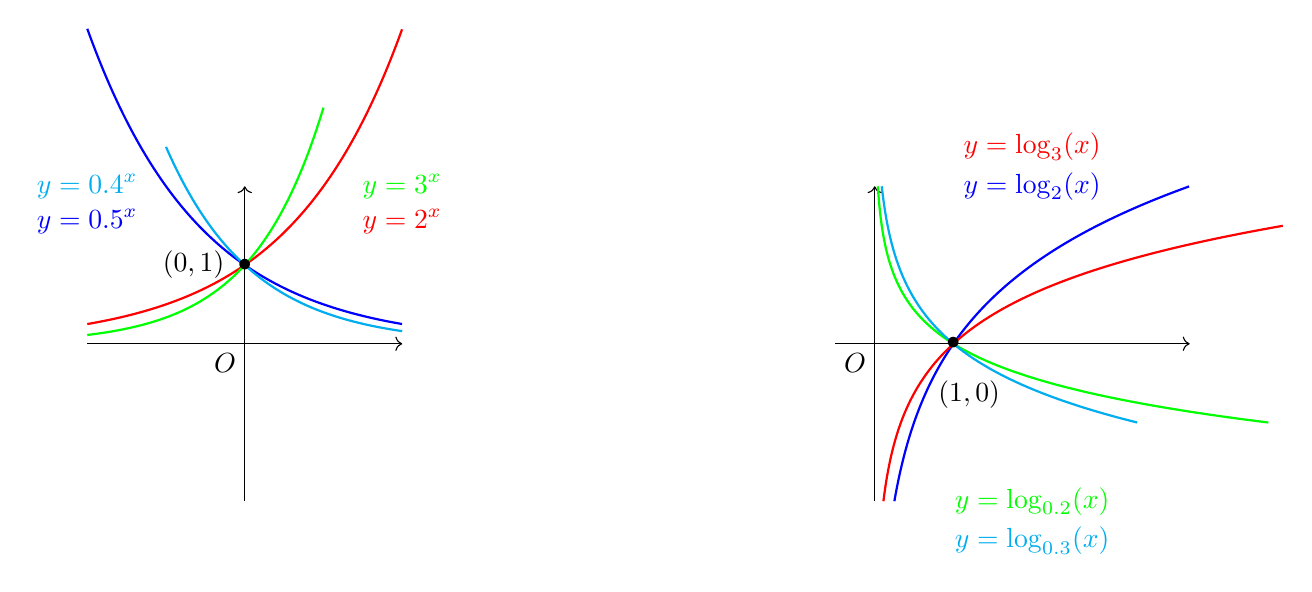
\begin{tikzpicture}
        \begin{scope}
            \draw [->](-2,0)--(2,0);
            \draw [->](0,-2)--(0,2);
            \node at (-.25,-.25){$O$};
            \draw[domain=-2:2, samples=1000, thick,color=red]
              plot(\x,{2^\x});
            \node[color=red] at (2,1.55){$\displaystyle y=2^{x} $};
            \draw[domain=-2:1, samples=1000, thick,color=green]
              plot(\x,{3^\x});
            \node[color=green] at (2,2){$\displaystyle y=3^{x} $};
            \draw[domain=-2:2, samples=1000, thick,color=blue]
              plot(\x,{0.5^\x});
            \node[color=blue] at (-2,1.55){$\displaystyle y=0.5^{x} $};
            \draw[domain=-1:2, samples=1000, thick,draw=cyan]
              plot(\x,{0.4^\x});
            \node[color=cyan] at (-2,2){$\displaystyle y=0.4^{x} $};
            \node at (0,1){$\bullet $};
            \node at (-.65,1){$(0,1)$};
        \end{scope} 
        \begin{scope}[xshift=8cm]
            \draw [->](-0.5,0)--(4,0);
            \draw [->](0,-2)--(0,2);
            \node at (-.25,-.25){$O$};
            \draw[domain=-2:2, samples=1000, thick,color=blue]
              plot({2^\x},\x);
            \node[color=blue] at (2,2){$\displaystyle y=\log _{2}(x) $};
            \draw[domain=-2:1.5, samples=1000, thick,color=red]
              plot({3^\x},\x);
            \node[color=red] at (2,2.5){$\displaystyle y=\log _{3}(x) $};
            \draw[domain=-1:2, samples=1000, thick,color=green]
              plot({0.2^\x},\x);
            \node[color=green] at (2,-2){$\displaystyle y=\log _{0.2}(x) $};
            \draw[domain=-1:2, samples=1000, thick,color=cyan]
              plot({0.3^\x},\x);
            \node[color=cyan] at (2,-2.5){$\displaystyle y=\log _{0.3}(x) $};
            \node at (1,0){$\bullet $};
            \node at (1.2,-.65){$(1,0)$};
        \end{scope}
    \end{tikzpicture}
    \caption{指数函数(左)对数函数(右)}
    \label{<label>}
\end{figure}

5、三角函数和反三角函数

三角函数

正弦,余弦,正切:
\begin{align}
    y&=\sin x  ,D_f=\mathbf{R} ,R_f= \left[1,1\right]     \\
    y&=\cos x  ,D_f=\mathbf{R} ,R_f= \left[1,1\right]     \\
    y&=\tan x=\frac{\sin x}{\cos x},D_f=x\neq \pm \frac{(2n-1)\pi}{2}(n=1,2\ldots ),R_f= \mathbf{R}   
\end{align}

正割,余割,余切:
\begin{align}
    y&=\sec x=\frac{1}{\cos x},D_f=x\neq \pm \frac{(2n-1)\pi}{2}(n=1,2\ldots ),R_f= \left(-\infty ,1 \right]\cup\left[1,+\infty \right)\\
    y&=\text{cse} x =\frac{1}{\sin x},D_f=x\neq \pm 2n\pi(n=0,1,2\ldots),R_f= \left(-\infty ,1 \right]\cup\left[1,+\infty \right)\\
    y&=\cot x=\frac{1}{\tan x},D_f=x\neq \pm 2n\pi(n=0,1,2\ldots),R_f= \mathbf{R}   
\end{align}

正弦、余弦、正割、余割的周期为$2\pi$,正切、余切的周期为$\pi$

正弦曲线
\begin{align}
    y=A\sin (\omega x+\varphi )
\end{align}

其他曲线同理。

$T=\frac{2\pi}{\omega },\varphi $是初相位.

三角公式:

公式1:

\begin{align}
    &\sin^2 x+\cos^2 x=1\\
    &1+\cot^2 x=\text{csc}^2 x\\
    &\tan^2 x +1=\sec^2 x
\end{align}

公式2:

\begin{align}
    \cos (A\pm B)&=\cos A \cos B \mp \sin A \sin B\\
    \sin (A\pm B)&=\sin A \cos B \pm\cos A \sin B\\
    \tan (A\pm B)&=\frac{\tan A \pm \tan B}{1\mp \tan A\tan B}
\end{align}

公式3(半角公式,变次公式)(正负号由$\theta $决定):

\begin{align}
    \cos ^{2}\theta &=\frac{1+\cos 2\theta }{2}\\
    \sin ^{2}\theta &=\frac{1-\cos 2\theta }{2}\\
    \tan ^{2}\theta &=(\frac{\sin \theta}{1+\cos \theta})^{2}=(\frac{1-\cos \theta}{\sin \theta})^{2}=\frac{1-\cos \theta}{1+\cos \theta}
\end{align}

公式4(倍角公式):
\begin{align}
    \sin 2\theta &=2\sin\theta \cos \theta =\frac{2\tan \theta}{1+\tan^{2}\theta}\\
    \cos 2\theta &=\cos ^{2}\theta -\sin ^{2}\theta =2\cos ^{2}\theta -1=1-2\sin^{2}\theta=\frac{1-\tan^{2}\theta}{1+\tan^{2}\theta}\\
    \tan 2\theta&=\frac{2\tan \theta}{1-\tan^{2}\theta}
\end{align}

公式5(和差化积):
\begin{align}
    \sin A\pm \sin B&=2\sin(\frac{A\pm B}{2})\cos(\frac{A\mp B}{2})\\
    \cos A+\cos B&=2\cos(\frac{A+B}{2})\cos(\frac{A-B}{2})\\
    \cos A-\cos B&=-2\sin(\frac{A+B}{2})\sin(\frac{A-B}{2})
\end{align}

公式6(积化和差):
\begin{align}
    \sin A\cos B&=\frac{1}{2}\left[\sin(A+B)+\sin(A-B)\right]\\
    \cos A\cos B&=\frac{1}{2}\left[\cos(A+B)+\cos(A-B)\right]\\
    \sin A\sin B&=\frac{1}{2}\left[\cos(A+B)-\cos(A-B)\right]
\end{align}

注意的是,一般只要背公式(32)(35)(36)就可以推导其他公式.

\begin{figure}[htb]
  \centering
  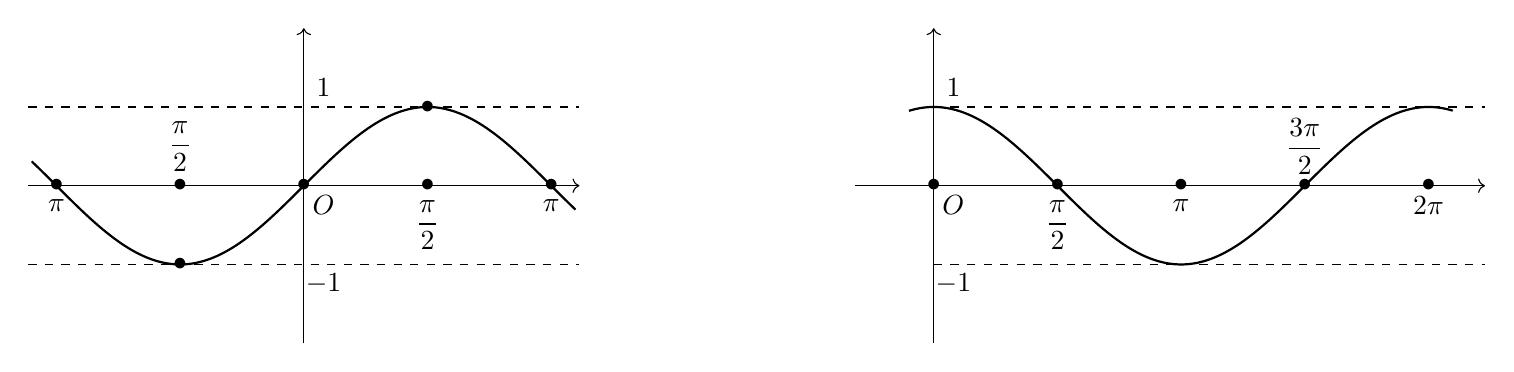
\begin{tikzpicture}
      \begin{scope}
          \draw [->](-3.5,0)--(3.5,0);
          \draw [->](0,-2)--(0,2);
          \draw [dashed](-3.5,1)--(3.5,1);
          \draw [dashed](-3.5,-1)--(3.5,-1);
          \node at (.25,-.25){$O$};
          \draw[domain=-pi-pi/10:pi+pi/10, samples=1000, thick]
              plot(\x,{sin (\x r)});
          \node at (0,0){$\bullet $};
          \node at (pi,0){$\bullet $};
          \node at (pi,-.25){$\pi $};
          \node at (pi/2,0){$\bullet $};
          \node at (pi/2,1){$\bullet $};
          \node at (pi/2,-.5){$ \displaystyle\frac{\pi}{2}$};
          \node at (-pi,0){$\bullet $};
          \node at (-pi,-.25){$\pi $};
          \node at (-pi/2,0){$\bullet $};
          \node at (-pi/2,.5){$\displaystyle\frac{\pi}{2} $};
          \node at (-pi/2,-1){$\bullet $};
          \node at (.25,1.25){$1 $};
          \node at (.25,-1.25){$-1 $};
      \end{scope} 
      \begin{scope}[xshift=8cm]
        \draw [->](-1,0)--(7,0);
        \draw [->](0,-2)--(0,2);
        \draw [dashed](0,1)--(7,1);
        \draw [dashed](0,-1)--(7,-1);
        \node at (.25,-.25){$O$};
        \draw[domain=-pi/10:pi+pi+pi/10, samples=1000, thick]
            plot(\x,{cos (\x r)});
        \node at (0,0){$\bullet $};
        \node at (pi,0){$\bullet $};
        \node at (pi,-.25){$\pi $};
        \node at (pi/2,0){$\bullet $};
        \node at (pi/2,-.5){$ \displaystyle\frac{\pi}{2}$};
        \node at (pi+pi,0){$\bullet $};
        \node at (pi+pi,-.25){$2\pi $};
        \node at (pi/2+pi,0){$\bullet $};
        \node at (pi/2+pi,.5){$\displaystyle\frac{3\pi}{2} $};
        \node at (.25,1.25){$1 $};
        \node at (.25,-1.25){$-1 $};
      \end{scope}
  \end{tikzpicture}
  \caption{正弦函数(左)、余弦函数(右)图像(部分)}
  \label{<label>}
\end{figure}

\begin{figure}[htb]
  \centering
  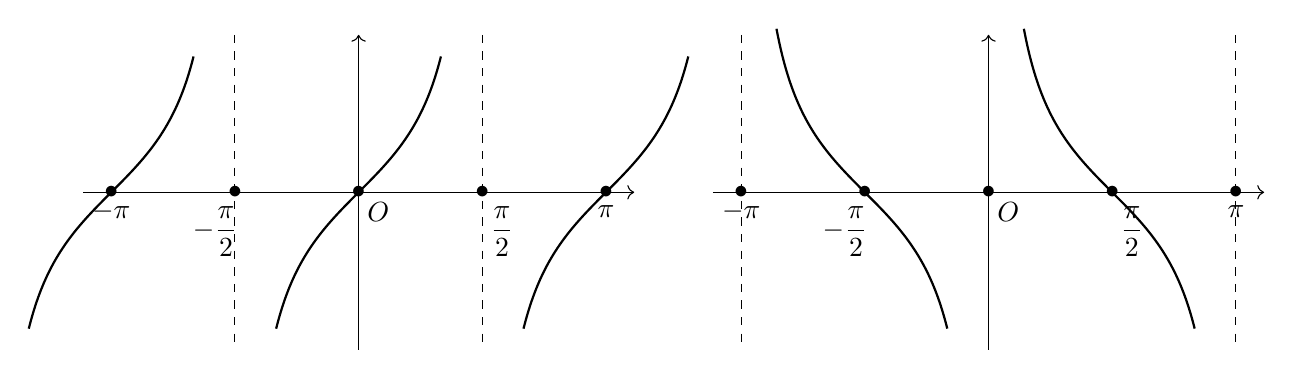
\begin{tikzpicture}
      \begin{scope}
          \draw [->](-3.5,0)--(3.5,0);
          \draw [->](0,-2)--(0,2);
          \draw [dashed](pi/2,2)--(pi/2,-2);
          \draw [dashed](-pi/2,2)--(-pi/2,-2);
          \node at (.25,-.25){$O$};
          \draw[domain=-pi/3:pi/3, samples=1000, thick]
              plot(\x,{tan (\x r)});
          \draw[domain=pi/3+pi/3:pi/3+pi, samples=1000, thick]
              plot(\x,{tan (\x r)});
          \draw[domain=-pi/3-pi:pi/3-pi, samples=1000, thick]
              plot(\x,{tan (\x r)}); 
          \node at (0,0){$\bullet $};
          \node at (pi,0){$\bullet $};
          \node at (pi,-.25){$\pi $};
          \node at (pi/2,0){$\bullet $};
          \node at (pi/2+.25,-.5){$ \displaystyle\frac{\pi}{2}$};
          \node at (-pi,0){$\bullet $};
          \node at (-pi,-.25){$-\pi $};
          \node at (-pi/2,0){$\bullet $};
          \node at (-pi/2-.25,-.5){$\displaystyle -\frac{\pi}{2} $};  
      \end{scope} 
      \begin{scope}[xshift=8cm]
        \draw [->](-3.5,0)--(3.5,0);
        \draw [->](0,-2)--(0,2);
        \node at (.25,-.25){$O$};
        \draw [dashed](pi,2)--(pi,-2);
        \draw [dashed](-pi,2)--(-pi,-2);
        \draw[domain=pi/7:pi/2+pi/3, samples=1000, thick]
            plot(\x,{cot(\x r) });
        \draw[domain=pi/7-pi:pi/2+pi/3-pi, samples=1000, thick]
            plot(\x,{cot(\x r) });
        \node at (0,0){$\bullet $};
        \node at (pi,0){$\bullet $};
        \node at (pi,-.25){$\pi $};
        \node at (pi/2,0){$\bullet $};
        \node at (pi/2+.25,-.5){$ \displaystyle\frac{\pi}{2}$};
        \node at (-pi,0){$\bullet $};
        \node at (-pi,-.25){$-\pi $};
        \node at (-pi/2,0){$\bullet $};
        \node at (-pi/2-.25,-.5){$\displaystyle -\frac{\pi}{2} $};   
      \end{scope}
  \end{tikzpicture}
  \caption{正切函数(左)、余切函数(右)图像(部分)}
  \label{<label>}
\end{figure}

\begin{figure}[htb]
  \centering
  \begin{tikzpicture}
      \begin{scope}
          \draw [->](-3.5,0)--(3.5,0);
          \draw [->](0,-2)--(0,2);
          \draw [dashed](pi/2,2)--(pi/2,-2);
          \draw [dashed](-pi/2,2)--(-pi/2,-2);
          \node at (.25,-.25){$O$};
          \draw [dashed](-3.5,1)--(3.5,1);
          \draw [dashed](-3.5,-1)--(3.5,-1);
          \node at (.25,1.25){$1 $};
          \node at (.25,-1.25){$-1 $};
          \draw[domain=-pi/3:pi/3, samples=1000, thick]
              plot(\x,{sec (\x r)});
          \draw[domain=-pi/3+pi:pi, samples=1000, thick]
              plot(\x,{sec (\x r)});
          \draw[domain=-pi:pi/3-pi, samples=1000, thick]
              plot(\x,{sec (\x r)});         
          \node at (0,0){$\bullet $};
          \node at (pi,0){$\bullet $};
          \node at (pi,-.25){$\pi $};
          \node at (pi/2,0){$\bullet $};
          \node at (pi/2+.25,-.5){$ \displaystyle\frac{\pi}{2}$};
          \node at (-pi,0){$\bullet $};
          \node at (-pi,-.25){$-\pi $};
          \node at (-pi/2,0){$\bullet $};
          \node at (-pi/2-.25,-.5){$\displaystyle -\frac{\pi}{2} $};  
      \end{scope} 
      \begin{scope}[xshift=8cm]
        \draw [->](-3.5,0)--(3.5,0);
        \draw [->](0,-2)--(0,2);
        \node at (.25,-.25){$O$};
        \draw [dashed](pi,2)--(pi,-2);
        \draw [dashed](-pi,2)--(-pi,-2);
        \draw [dashed](-3.5,1)--(3.5,1);
        \draw [dashed](-3.5,-1)--(3.5,-1);
        \node at (.25,1.25){$1 $};
        \node at (.25,-1.25){$-1 $};
        \draw[domain=pi/8:pi/2+pi/3+pi/100, samples=1000, thick]
            plot(\x,{sin(\x r)^-1 });
        \draw[domain=pi/8-pi:-pi/2+pi/3+pi/100, samples=1000, thick]
            plot(\x,{sin(\x r)^-1 });            
        \node at (0,0){$\bullet $};
        \node at (pi,0){$\bullet $};
        \node at (pi,-.25){$\pi $};
        \node at (pi/2,0){$\bullet $};
        \node at (pi/2+.25,-.5){$ \displaystyle\frac{\pi}{2}$};
        \node at (-pi,0){$\bullet $};
        \node at (-pi,-.25){$-\pi $};
        \node at (-pi/2,0){$\bullet $};
        \node at (-pi/2-.25,-.5){$\displaystyle -\frac{\pi}{2} $};   
      \end{scope}
  \end{tikzpicture}
  \caption{正切函数(左)、余切函数(右)图像(部分)}
  \label{<label>}
\end{figure}

\newpage

反三角函数

将三角函数的定义域进行限制,我们就可以定义出三角函数的反函数,我们称之为反三角函数.

正弦函数$\displaystyle y=\sin x ,x\in \left[-\frac{\pi}{2},\frac{\pi}{2}\right] \Longrightarrow $反正弦函数$\displaystyle y=\arcsin x,x\in \left[-1,1\right] ,y\in\left[-\frac{\pi}{2},\frac{\pi}{2}\right] $\\

余弦函数$\displaystyle y=\cos x ,x\in \left[0,\pi\right] \Longrightarrow $反余弦函数$\displaystyle y=\arccos x,x\in \left[-1,1\right] ,y\in\left[0,\pi\right] $\\

正切函数$\displaystyle y=\tan x ,x\in (-\frac{\pi}{2},\frac{\pi}{2}) \Longrightarrow $反正切函数$\displaystyle y=\arctan x,x\in \mathbf{R}  ,y\in (-\frac{\pi}{2},\frac{\pi}{2}) $\\

余切函数$\displaystyle y=\cot x ,x\in (-\frac{\pi}{2},\frac{\pi}{2}) \Longrightarrow $反余切函数$\displaystyle y=\text{arccot} x,x\in \mathbf{R}  ,y\in (0,\pi ) $\\

\begin{figure}[htb]
  \centering
  \begin{tikzpicture}
      \begin{scope}
          \draw [->](-2,0)--(2,0);
          \draw [->](0,-2)--(0,2);
          \draw [dashed](-2,pi/2)--(2,pi/2);
          \draw [dashed](-2,-pi/2)--(2,-pi/2);
         
          \node at (.25,-.25){$O$};
          \node at (0,pi/2){$\bullet $};
          \node at (0,-pi/2){$\bullet $};
          \node at (.25,pi/2){$\displaystyle\frac{\pi}{2}$};
          \node at (.25,-pi/2){$\displaystyle -\frac{\pi}{2} $};
          \node at (1,-.25){$1$} ;
          \node at (1,0){$\bullet $};
          \node at (-1,-.25){$-1$} ;
          \node at (-1,0){$\bullet $};
          \draw[domain=-pi/2:pi/2, samples=1000, thick]
              plot({sin (\x r)},\x);
           
      \end{scope} 
      \begin{scope}[xshift=8cm,yshift=-1.48cm]
        \draw [->](-2,0)--(2,0);
        \draw [->](0,-1)--(0,3.5);
        \node at (.25,-.25){$O$};
        \draw [dashed](2,pi)--(-2,pi);
        \node at (0,pi){$\bullet $};
        \node at (.25,pi+.2){$\pi$};
        \node at (.25,pi/2+.2){$\displaystyle\frac{\pi}{2}$};
        \node at (0,pi/2){$\bullet $}; 
        \node at (1,-.25){$1$} ;
        \node at (1,0){$\bullet $};  
        \draw[domain=0:pi, samples=1000, thick]
            plot({cos(\x r) },\x);
                    
        
      \end{scope}
  \end{tikzpicture}
  \caption{反正弦函数函数(左)、反余弦函数(右)图像}
  \label{<label>}
\end{figure}

\begin{figure}[htb]
  \centering
  \begin{tikzpicture}
      \begin{scope}
          \draw [->](-2,0)--(2,0);
          \draw [->](0,-2)--(0,2);
          \draw [dashed](-2,pi/2)--(2,pi/2);
          \draw [dashed](-2,-pi/2)--(2,-pi/2);
         
          \node at (.25,-.25){$O$};
          \node at (0,pi/2){$\bullet $};
          \node at (0,-pi/2){$\bullet $};
          \node at (.25,pi/2){$\displaystyle\frac{\pi}{2}$};
          \node at (.25,-pi/2){$\displaystyle -\frac{\pi}{2} $};
          \node at (1,-.25){$1$} ;
          \node at (1,0){$\bullet $};
          \node at (-1,-.25){$-1$} ;
          \node at (-1,0){$\bullet $};
          \draw[domain=-pi/3:pi/3, samples=1000, thick]
              plot({tan (\x r)},\x);
           
      \end{scope} 
      \begin{scope}[xshift=8cm,yshift=-1.48cm]
        \draw [->](-2,0)--(2,0);
        \draw [->](0,-1)--(0,3.5);
        \node at (.25,-.25){$O$};
        \draw [dashed](2,pi)--(-2,pi);
        \node at (0,pi){$\bullet $};
        \node at (.25,pi+.2){$\pi$};
        \node at (.25,pi/2+.2){$\displaystyle\frac{\pi}{2}$};
        \node at (0,pi/2){$\bullet $}; 
        \node at (1,-.25){$1$} ;
        \node at (1,0){$\bullet $};  
        \draw[domain=pi/10:pi-pi/10, samples=1000, thick]
            plot({cot(\x r) },\x);
                    
        
      \end{scope}
  \end{tikzpicture}
  \caption{反正切函数函数(左)、反余切函数(右)图像(部分)}
  \label{<label>}
\end{figure}

\newpage

其他函数(主要是绝对值函数,)

a.绝对值函数
$f(x)=\left\lvert x\right\rvert =\begin{dcases}
x,&x>0;\\-x,&x<0.    
\end{dcases}$%列式子
范围
$\begin{dcases}
D=R\\R_f=\left[0,\infty \right)%半开半闭区间
\end{dcases}$%表示定义域和值域

同时绝对值还表示两点的距离(重点)

\begin{figure}[htbp]%绝对值函数图像,文章中
    \centering
\begin{tikzpicture}[>=latex]
  \begin{scope}
   \draw[->](-3,0)--(3,0)node[right]{$x$};%画x轴
\draw[->](0,-1)--(0,3)node[right]{$y$};%画y轴
\draw(0,0)--(2,2);
\draw(0,0)--(-2,2)node[left]{$\vert x\vert $};
\draw(-.2,-.2)node{$O$};%表明原点

   \end{scope}             
   \begin{scope}[xshift=8cm]
   \draw[->](-2,0)--(2,0)node[right]{$x$};
   \draw[->](0,-2)--(0,2)node[right]{$y$};
   \draw(0,1)node[left]{$1$}--(2,1);
   \draw(0,1)node{$\circ $};
  \draw(0,-1)node[right]{$-1$}--(-2,-1);
  \draw(0,-1)node{$\circ $};
  \draw(-0.2,-0.2)node{$O$};
  \draw(0,0)node{$\bullet $};
                
    
  \end{scope}
  
\end{tikzpicture}
\caption{绝对值函数(左)、符号函数函数(右)图像(部分)}
\end{figure}

b.符号函数
$f(x)=\text{sgn} x=\begin{dcases}
    -1,&x<0;\\0,&x=0;\\1,&x>0.
\end{dcases}$
范围
$\begin{dcases}
D=R\\R_f=\{-1,0,1\}
\end{dcases}$

注意:$\text{sgn} x\cdot |x| =x$\\

c.取整函数

我们将不超过$x$的最大整数称为$x$的整数部分称为$x$的整数,可定义函数$f(x)=[x]$,该函数称为取整函数,其图像称为阶梯曲线.


\begin{figure}[htbp]
    \centering
\begin{tikzpicture}
\draw[->](-2,0)--(3,0)node[right]{$x$};
\draw[->](0,-2)--(0,3)node[right]{$y$};
\foreach \x in{-1,1,2}
{
    \draw (0,\x)node[left]{$\x$}--(.1,\x);
    \draw (\x,0)node[below]{$\x$}--(\x,.1);
}%画刻度
\draw(1,1)node{$\bullet $}--(2,1)node{$\circ $};
\draw(0,0)node{$\bullet $}--(1,0)node{$\circ $};
\draw(-1,-1)node{$\bullet $}--(0,-1)node{$\circ $};
\draw(-0.2,-0.2)node{$O$};
\end{tikzpicture}
    \caption{取整函数}
\end{figure}

狄利克雷函数
$D(x) = 
\begin{dcases}
  1,&x \in Q;\\0,&x \in Q^c.    
  \end{dcases}$
$Q^c$是无理数

$\forall r \in R$是其周期,所以该函数无最小正周期.

邻域(了解就好,因为后面会涉及到所以就讲一下)

以$x_{0}$为中心的$\forall $开区间称为点$x_{0}$的邻域,记作$\bigcup (x_{0})$,在$\bigcup (x_{0})$中去掉中心$x_{0}$后,称为点$x_{0}$的去心邻域,记作$\bigcup \limits^{\circ }(x_{0})$

设$x_{0}\in \mathbf{R} ,\delta >0$,开区间$(x_{0}-\delta ,x_{0}+\delta ) $称为点$x_{0}$的$\delta $邻域,记作$\bigcup (x_{0},\delta )$,在$\bigcup (x_{0},\delta )$中去掉中心$x_{0}$后,称为点$x_{0}$的去心$\delta $邻域,记作$\bigcup \limits^{\circ }(x_{0},\delta )$

\newpage 

\subsection{\heiti 数列极限}

一、数列极限的定义

数列$\left\{x_{n}\right\} $,常数$a$,$\forall \varepsilon >0$,$\exists N\in  N_{+}$,当$n>N$时,有$|x_{n}-a|<\varepsilon .\Leftrightarrow \lim\limits_{n\to \infty }x_{n}=a .$

反之发散.

直观上,当$n\to \infty $时,数列非常靠近某个数$a$,那么数列极限收敛于$a$ ,反之发散.

二、数列极限的性质

1、唯一性:数列$x_{n}$极限收敛$\Leftrightarrow $数列$x_{n}$极限是唯一的.

2、有界性:数列$x_{n}$极限收敛$\Rightarrow $数列$x_{n}$一定有界(例如$x_{n}=(-1)^{n}$).

3、保号性:如果$\lim \limits_{n\to \infty}x_{n}=a>0(<0)$,那么$\exists N\in N_{+}$当$n>N$时,都有$x_{n}>0(<0)$.

推论:如果数列$x_{n}$从某项起有$x_{n}\geqslant 0(\leqslant 0)$,且$\lim \limits_{n\to \infty}x_{n}=a$,那么$a>0(<0)$

4、数列$x_{n}$收敛于$a\Rightarrow $其任意子数列都收敛于$a$.

推论:数列$x_{n}$的一个子数列发散或者两个子数列收敛于不同的极限$\Leftrightarrow $数列$x_{n}$发散.

结论:对于性质四我们一般取数列的奇数项和偶数项来判断数列极限是否收敛.

\subsection{\heiti 函数的极限}

一、函数极限的定义

(1)自变量趋于有限值时
\begin{align}
    \lim\limits_{x\to x_{0}}f(x)=A\Leftrightarrow  \forall \varepsilon >0,\exists \delta >0,\text{当}0<|x-x_{0}|<\delta \text{时,有}|f(x)-A|<\epsilon.
\end{align}

当$\lim f(x)=\infty$时,函数极限不存在

(2)自变量趋于无穷时
\begin{align}
    \lim\limits_{x\to\infty }f(x)=A\Leftrightarrow \forall X >0,\exists \delta >0,\text{当}|x|>X \text{时,有}|f(x)-A|<\epsilon.
\end{align}

当$\lim f(x)=\infty$时,函数极限不存在

(3)单侧极限的定义

左极限的定义:
\begin{align}
    f(x^{-}_{0})=\lim\limits_{x\to x_{0}^{-}}f(x)=A\Leftrightarrow \forall \varepsilon >0,\exists\delta >0 ,\text{当} x_{0}-\delta <x<x_{0}\text{时,有}|f(x)-A|<\varepsilon \text{其中}x\text{恒小于}x_0
\end{align}

右极限的定义:
\begin{align}
    f(x^{+}_{0})=\lim\limits_{x\to x_{0}^{+}}f(x)=A\Leftrightarrow \forall \varepsilon >0,\exists \delta>0 ,\text{当} x_{0}<x<x_{0}+\delta \text{时,有}|f(x)-A|<\varepsilon .\text{其中}x\text{恒大于}x_0
\end{align}

当$ f(x^{-}_{0})$和$f(x^{+}_{0})$存在,且$f(x^{+}_{0})= f(x^{-}_{0}   )=A$时,$\lim\limits_{x\to x_{0}}f(x)=A$

我们经常用用这个方法来判断函数极限是否存在.(尤其是分段函数)

$\lim\limits_{x\to x_{0}} f(x)=A\Leftrightarrow \lim\limits_{x\to x_{0}^{+}}f(x)=\lim\limits_{x\to x_{0}^{-}}f(x)=A$

$\lim\limits_{x\to \infty }f(x)=A\Leftrightarrow \lim\limits_{x\to +\infty }f(x)=\lim\limits_{x\to -\infty }f(x)=A$

二、函数极限的性质

(1)函数极限的唯一性

$\displaystyle \lim f(x)=A\Leftrightarrow A\text{唯一};$

(2)函数极限的局部有界性

$\lim f(x)=A,\exists \text{常数}M>0\text{和}\delta >0,\text{使得当}0<|x-x_{0}|<\delta \text{时,有}|f(x)|\leqslant M$

(3)函数极限的局部保号性

$\lim f(x)=A>0(<0),\exists \text{常数}\delta >0,\text{使得当}0<|x-x_{0}|<\delta \text{时,有}f(x)>0(<0)$

    推论:如果在$\bigcup \limits^{\circ }(x_{0} )$内,$f(x)\geqslant 0(\leqslant 0)$,而且$\lim \limits_{x \to x_{0}}f(x)=A$,那么$A\geqslant 0(\leqslant 0)$

(4)函数极限与数列极限的关系

$\text{如果}\exists \text{极限}\lim\limits_{x\to x_{0}} f(x),\{x_{n}\}\text{为函数}f(x)\text{的定义域内任意收敛于}x_{0}\text{的数列},\text{且满足}x_{n}\neq x_{0},\text{那么相应的函数值数列}\{f(x_{n})\}\text{必收敛,且}\lim\limits_{n\to\infty }f(x_{n})=\lim\limits_{x\to x_{0} }f(x)$

\subsection{\heiti无穷大与无穷小}

一.无穷小

定义:$\lim f(x)=0$.

特别的$\lim \limits _{n\to \infty }x_n=0$,称为$\{x_n\}$在$n \to \infty$时的无穷小.

定理1:$\lim f(x)= A\Longleftrightarrow f(x)=A+\alpha ,\lim\alpha =0$.

二.无穷大

定义:$\lim f(x)=\infty $.

定理2:极限状态下,在$x$同一变化过程中$\displaystyle 0=\frac{1}{\infty}$或$\displaystyle \infty=\frac{1}{0}$.

\subsection{\heiti极限运算法则}

定理1:有限个无穷小之和是无穷小;

定理2:有界函数与无穷小乘积是无穷小;

推论1:常数与无穷小乘积是无穷小;

推论2:有限个无穷小的乘积是无穷小;

定理3:在$x$的同一变化过程中,如果$\lim f(x)=A$,$\lim g(x)=B$,则有

\begin{align*} 
    \lim [f(x)\pm g(x)]&=\lim f(x)\pm \lim g(x)=A\pm B \\
    \lim [f(x)\cdot g(x)]&=\lim f(x)\cdot \lim g(x)=A\cdot B\\
    \displaystyle\lim \frac {f(x)}{g(x)} &= \frac{\lim f(x)}{\lim g(x)}=\frac{A}{B}(B\neq 0)\\
\end{align*}

推论3:若$\lim f(x)$存在,C为常数.则$\lim Cf(x)=C\lim f(x)$

推论4:若$\lim f(x)$存在,$n \in Z^+$,那么$\lim \left[f(x)\right]^n=\left[\lim f(x)\right]^n$;

定理4:如果$f(x)\geqslant g(x)$,而$\lim f(x)=A$,$\lim g(x)=B$,那么$A\geqslant B$

定理5:设$\lim f\left[g(x)\right]=\lim f\left[\lim g(x)\right]$

求函数极限方法①

(1)对于多项式函数
\begin{align*}
    f(x)=\sum \limits_{i=0}^{n} a_{i}x^{n-i}(n-i>0,n\in \mathbf{Z} )
\end{align*}

我们一般直接带入,若自变量趋于无穷,函数也趋于无穷

(2)对有理函数
\begin{align*}
    \displaystyle f(x)=\frac{P(x)}{Q(x)}
\end{align*}
$P(x),Q(x)$是多项式函数

若$Q(x)\nrightarrow  0(\infty )$,那么则直接带入.

若$Q(x)\rightarrow  0(\infty )$,则分子分母同除最高次项然后带入.

$\displaystyle \lim\limits_{x\to \infty }f(x)=\lim\limits_{x\to \infty }\frac{P(x)}{Q(x)}=\lim\limits_{x\to \infty }\displaystyle \frac{\sum \limits_{i=0}^{m} b_{i}x^{m-i}}{\sum \limits_{i=0}^{n} a_{i}x^{n-i}}=
\begin{dcases}
    \infty  \ \ m>n\\
    \displaystyle\frac{b_{0}}{a_{0}}\ \ m=n\\
    \ 0  \ \ \ m<n
\end{dcases}$

当然遇到只有根式(没有分式)的时候,分子分母同乘共轭式,同除最高次项把每一项化成分式

若$\lim f(x)=A>0,\lim g(x)=B.A,B$为常数,则$\displaystyle\lim f(x)^{g(x)}=\lim f(x)^{\lim g(x)}=A^{B}$

若$\lim f(x)=A>0,\lim g(x)=+\infty$为常数,则$\displaystyle\lim f(x)^{g(x)}=
\begin{dcases}
0(0<A<1) \\ \infty(A>1)   
\end{dcases}$

\subsection{\heiti极限存在准则,两个重要极限}
一.极限存在准则

准则1:$\left\{x_n\right\} $、$\left\{y_n\right\}$、$\left\{z_n\right\}$满足:

(1)$\exists n_0\in N_+$,当$n>n_0$时有$y_n\leq x_n\leq z_n$;

(2)$\lim\limits_{n\to \infty} y_n=\lim\limits_{n\to \infty} z_n=a$;

则$\lim \limits_{n\to \infty}x_n=a$.

准则1':$f(x) $、$g(x)$、$h(x)$满足:

(1)$\bigcup \limits ^{\circ}(x_0)$(或$\left\lvert x\right\rvert>M $)时有$g(x)\leq f(x)\leq h(x)$;

(2)$\lim g(x)=\lim h(x)=A$;

则$\lim f(x)=A$.

重要极限1:$x\in \left(0,\frac{\pi}{2}\right) $时有

\begin{align}
    \displaystyle \lim \limits_{x\to 0}\frac{\sin x}{x}=1.
\end{align}

准则2:单调有界,必有极限.

重要极限2:

\begin{align}
   \displaystyle \lim \limits_{x\to \infty}(1+f(x))^{\frac{1}{f(x)}}=e 
\end{align}

其中$\lim f(x)=0$.

大多数情况要配凑

常见配凑:$\displaystyle\lim\limits_{x\to \infty}(1+\displaystyle\frac{1}{x})^{x}=e\ \ \ \lim\limits_{x\to 0}(1+x)^{\frac{1}{x}}=e\ \ \ \lim\limits_{x\to \infty}(1-\frac{1}{x})^{ x}=\frac{1}{e}$

\subsection{\heiti无穷小的比较}

就是哪个函数能更快到达0

定义:

(1)$\displaystyle\lim \frac{\beta}{\alpha}  =0$时,$\beta $是比$\alpha $高阶的无穷小,记作:$\beta =\circ (\alpha )$;
\\

(2)$\displaystyle\lim \frac{\beta}{\alpha}=\infty$时,$\beta $是比$\alpha $低阶的无穷小;
\\

(3)$\displaystyle\lim \frac{\beta}{\alpha} =C\neq 0$时,$\beta $与$\alpha $同阶无穷小;
\\

(4)$\displaystyle\lim \frac{\beta}{\alpha ^k} =C\neq 0$时,$\beta $是关于$\alpha $的$k$阶无穷小;
\\

(5)$\displaystyle\lim \frac{\beta}{\alpha} =1$时,$\beta $与$\alpha $是{\heiti 等价无穷小},记作$\alpha \thicksim \beta $.
\\

定理1:$\alpha \thicksim \beta \Leftrightarrow \beta = \alpha +\circ (\alpha )$.
\\

定理2:$\alpha \thicksim \tilde{\alpha } $、$\beta  \thicksim \tilde{\beta } $,且$\displaystyle \lim \frac{\tilde{\alpha }}{\tilde{\beta }}$存在,则$\displaystyle \lim \frac{\alpha }{\beta}=\lim \frac{\tilde{\alpha }}{\tilde{\beta }}$.
\\

性质1:$\alpha \thicksim \beta \Leftrightarrow \beta \thicksim \alpha $.

性质2:$\alpha \thicksim \alpha $.

性质3:$\alpha \thicksim \beta$,$\beta \thicksim \gamma \Leftrightarrow \alpha \thicksim  \beta \thicksim  \gamma $

常见的等价无穷小

\begin{tabular}{|c|c|c|}
    \hline
    $\sin x\thicksim x$&$\arcsin  x\thicksim x$&$\tan x\thicksim x$\\
    \hline
    $\arctan x\thicksim x$&$\log_{a}x\thicksim\frac{x}{\ln a}$&$\ln (1+x)\thicksim x$\\
    \hline
    $\alpha ^x-1\thicksim x\ln \alpha$&  $e^x-1 \thicksim x$&$ 1-\cos x\thicksim \frac{x^2}{2}$\\
    \hline
    $x-\sin x\thicksim \frac{x^3}{6}$&$\tan x -x\thicksim \frac{x^3}{3}$ &$(1+x)^\alpha -1\thicksim \alpha x$\\
    \hline
    $\arcsin x-x\thicksim \frac{x^3}{6}$&$x-\arctan  x\thicksim \frac{x^3}{3}$&$\tan x-\sin x\thicksim \frac{x^3}{2}$\\
    \hline
\end{tabular}

\subsection{\heiti函数的连续性与间断点}

一.连续性

定义:设$y=f(x)$在$\bigcup \limits ^{\circ}(x_0)$内有定义,如果$\Delta y=\lim \limits_{\Delta x\to 0 }\left[f(x_0+\Delta x)-f(x_0)\right]=0 $或$y=\lim \limits_{x\to x_0}f(x)=f(x_0)$,那么称函数$y=f(x)$在点$x_0$连续.

如果$\lim \limits_{x\to x_0^-}f(x)=f(x_0)$存在,且$f(x_0^-)=f(x_0)$,那么$f(x)$在$x_0$点左连续;

如果$\lim \limits_{x\to x_0^+}f(x)=f(x_0)$存在,且$f(x_0^+)=f(x_0)$,那么$f(x)$在$x_0$点右连续.

若$f(x_0^+)=f(x_0^-)=f(x_0)$,则函数$y=f(x)$在点$x_0$连续.

连续函数的图形时连续不间断的曲线.

二.间断点

(1)第一类间断点

若$f(x)$在$x_0$处无定义,且$\lim\limits_{x\to x_0} f(x)$存在$\Leftrightarrow x_0$是$f(x)$可去间断点;

若$f(x)$在$x_0$处有定义,且$\lim\limits_{x\to x_0}  f(x)$不存在$\Leftrightarrow x_0$是$f(x)$跳跃间断点;

(2)第二类间断点

若$\lim \limits_{x\to x_0}f(x)=\infty \Leftrightarrow x_0$是$f(x)$无穷间断点;

若$f(x)$在$x_0$处有无定义,且$f(x)$在$\bigcup \limits ^{\circ}(x_0)$内快速变化$\Leftrightarrow x_0$是$f(x)$振荡间断点;

\subsection{\heiti连续函数的运算和初等函数的连续性}

一.连续函数的和差积商复合的连续性

定理1:$f(x)$、$g(x)$是连续函数,那么它们的和、差、积、商、复合运算后连续.

定理2:$f(x)$单调连续,则$f^{-1}(x)$也单调连续.

二.初等函数的连续性

初等函数在其定义区间内都是连续的.

\subsection{\heiti 闭区间上连续函数的性质}

一.有界性与最值定理

最大值定义:
$f(x)$在区间$I$上有定义,如果有$x\in I$,对$\forall x\in I$,都有$f(x_0)>f(x)$(或$f(x_0)<f(x)$)那么$f(x_0)$是$f(x)$的最大值(或最小值).

定理1:在闭区间上连续的函数在该区间上有界,一定能取到最值.

定理2:$f(x)$在$\left[a,b\right]$连续,$f(a)\cdot f(b)<0$,则$\exists $至少一个$c\in (a,b)$使$f(c)=0$.

定理3:$f(x)$在$\left[a,b\right]$连续,且$f(a)=A$、$f(b)=B$.设$C\in (A,B)$,那么$\exists $至少一个$c\in (a,b)$使$f(c)=C$.

推论:$f(x)$在$\left[a,b\right]$连续,值域为$\left[m,M\right]$,那么$m$、$M$是$f(x)$在$\left[a,b\right]$的最小值与最大值.


\newpage

\section{\heiti导数与微分}

\subsection{\heiti 导数的概念}

一.导数的定义

(1)$f(x)$在$x_0$处的导数

定义:$\displaystyle f^{\prime}(x_0)=\lim \limits_{\Delta x \to 0}\frac{\Delta y}{\Delta x}=\lim \limits_{\Delta x \to 0}\frac{f(x_0+\Delta x)-f(x_0)}{\Delta x}$.
\\

可记作$\displaystyle y^\prime |_{x=x_0}$、$\displaystyle \frac{dy}{dx}|_{x=x_0} $、$\displaystyle \frac {df(x)}{dx}|_{x=x_0}$.
\\

常见形式有$\displaystyle f^{\prime}(x_0)=\lim \limits_{x \to x_0}\frac{f(x)-f(x_0)}{x-x_0}$、$\displaystyle f^{\prime}(x_0)=\lim \limits_{h \to 0}\frac{f(x_0+h)-f(x_0)}{h}$.
\\

极限不存在,则导数不存在.若$y^\prime =\infty$,则说明函数$f(x)$在$x_0$处的导是无穷大.

(2)$f(x)$的导函数

$\displaystyle f^{\prime}(x)=\lim \limits_{\Delta x \to 0}\frac{f(x+\Delta x)-f(x)}{\Delta x}$、$\displaystyle f^{\prime}(x)=\lim \limits_{h \to 0}\frac{f(x+h)-f(x)}{h}$.
\\

记作$f^{\prime}(x)$、$y^\prime$、$\displaystyle \frac{d y}{d x} $、$\displaystyle \frac{d f(x)}{d x} $
\\

所以有$f^{\prime}(x_0)=f^{\prime}(x)|_{x=x_0}$
\\

(3)单侧导数

左导数$\displaystyle f^{\prime}_{-}(x_0)=\lim \limits_{h \to 0^-}\frac{f(x_0+h)-f(x_0)}{h}$;右导数$\displaystyle f^{\prime}_{+}(x_0)=\lim \limits_{h \to 0^+}\frac{f(x_0+h)-f(x_0)}{h}$;
\\

$f^{\prime}_{-}(x_0)=f^{\prime}_{+}(x_0) \text{且存在} \Leftrightarrow f^{\prime}(x)$在$x_0$处可导.$f^{\prime}_{+}(x_0)$、$f^{\prime}_{-}(x_0)$统称单侧导数.

如果$f(x)$在$(a,b)$可导,且$f^{\prime}_{+}(a)$、$f^{\prime}_{-}(b)$都存在,那么说$f(x)$在$\left[a,b\right] $上可导.

三.导数的几何意义

(1)斜率\ \ \ \ $k=f^{\prime}(x_0)=\tan \theta $

(2)切线方程\ \ \ \ $y-y_0=f^{\prime}(x_0)(x-x_0)$
\\

(3)法线\ \ \ \ $\displaystyle -\frac{1}{f^{\prime}(x_0)}$
\\

(4)法线方程\ \ \ \ $\displaystyle y-y_0=-\frac{1}{f^{\prime}(x_0)}(x-x_0) $
\\

注意:$f^{\prime}(x_0)=\infty\Leftrightarrow \text{切线是}x=x_0$

四.可导与连续

可导必连续,连续不一定可导.

\subsection{\heiti 求导法则}

一.函数的和差积商求导法则

如果$f(x)$和$g(x)$在$x$处有导数,那么其和差积商在$x$处有导数.\\


$\left[f(x)\pm g(x)\right]^\prime = f^\prime (x) \pm g^\prime (x)$

$\left[f(x)\cdot g(x)\right]^\prime = f^\prime (x) \cdot g (x)+f^\prime (x) \cdot g^\prime (x)$特别的$(Cf(x))^\prime =Cf^\prime (x)$\\

$\displaystyle  \left[\frac{f(x)}{g(x)}\right]^\prime = \frac{ f^\prime (x) \cdot g (x) - f(x) \cdot g^\prime (x)}{g^2(x)}$\\

二.反函数的求导法则\\

$\displaystyle \left[f^-1(x)\right]^\prime = \frac{1}{f(y)} $或$\displaystyle \frac{dy}{dx}= \frac{1}{ \dfrac{dx}{dy}}$\\


即反函数的导数是直接函数的导数的倒数.

三.复合函数求导法则

$y=\left[f\circ g(x)\right]$的导数为$\displaystyle \frac{dy}{dx} =\left[f\circ g(x)\right]^\prime =f^\prime  \left[g(x)\right]\cdot g^\prime (x) $或$\displaystyle \frac{dy}{dx}={\dfrac{dy}{dg(x)}}\cdot {\dfrac{dg(x)}{dx}}$\\

四.基本公式

\begin{tabular}{|c|c|c|}
    \hline
    $(C)^\prime =0$&$(x^{\mu })^\prime=\mu x^{\mu -1}$&$(\sin x)^\prime=\cos x$\\
    \hline
    $(\cos x)^\prime=-\sin x$&$(\tan x)^\prime=\sec^{2} x$&$(\cot x)^\prime=\csc^{2} x$\\
    \hline
    $(\sec x)^\prime=\sec x\cdot  \tan x$&$(\csc x)^\prime=-\csc x\cdot  \cot x$&$(a^x)^\prime=a^x\cdot \ln a (a>0,a\neq 1)$\\
    \hline
    $(e^{x})^\prime=e^{x}$&$(\log_{a}x)^\prime= -\frac{1}{x\ln a}$&$(\ln x)^\prime=\frac{1}{x} $\\
    \hline
    $(\arcsin x)^\prime=\frac{1}{\sqrt{1-x^{2}}}$&$(\arccos x)^\prime=-\frac{1}{\sqrt{1-x^{2}}}$&$(\arctan x)^\prime=\frac{1}{1+x^{2}}$\\
    \hline
    $(\text{arccot} x)^\prime=-\frac{1}{1+x^{2}}$& &\\
    \hline
\end{tabular}

\subsection{\heiti 高阶导数}

二阶及二阶以上的导数统称高阶导数,即$f^{\left(n\right)}(x)=y^{(n)}$(注意这个括号)如$y^{\prime \prime}=(y^\prime)^\prime$.

$\displaystyle (e^x)^{(n)}=e^x\ \ \ \ (\sin x )^{(n)}=\sin (x+\frac{n\pi}{2})\ \ \ \ (\cos x )^{(n)}=\cos (x+\frac{n\pi}{2})$

$\displaystyle \left[ln(1+x)\right]^{(n)} = (-1)^{n-1}\frac{(n-1)!}{(1+x)^n}\ \ \ \ (x^n)^{(n)}=n!\ \ \ \ (x^n)^{(n+1)}=0$

$\displaystyle (uv)^{(n)}=\sum \limits_{k=0}^{n}C^{k}_{n}u^{(n-k)}v^{(k)}$

\subsection{\heiti 隐函数求导及由参数方程说确定的函数的导数与相关变化率}

一.显隐函数

$f(x)$是显函数,$g(x,y)=0$是隐函数,将隐函数转换为显函数的过程叫显化.

令$y=y(x)$然后对方程两边同时求导;行求导.对于一些不容易直接求导的方程,可以两边先取对数再进

流程:求导$\to $归边$\to$带入$y\to$化简

技巧:$y=u^v=\text{e}^{v\ln u}$

二.参数方程的导

$\begin{dcases}
    y=f(t)\\x=g(t)
    \end{dcases}$
\ \ \ \ 其一阶导为$\displaystyle \frac{dy}{dx} =\frac{\dfrac{dy}{dt} }{\dfrac{dx}{dt} } =\dfrac{f^\prime (t)}{g^\prime (t)} $ .二阶导为$\displaystyle \frac{d^2 y}{d x^2}= \frac{ f^{(2)} (t) g^\prime (t) - f(x)^\prime  g^{(2)}(t)}{\left[g^\prime (t)\right]}$\\

\subsection{\heiti 函数的微分}

一.定义

设$y=f(x)$在某区间内有定义,$x_0$或$x_0+\Delta x$在这区间内,如果函数的增量$\Delta y= f(x_0+\Delta x)-f(x_0)$可表示为$\Delta y=A\Delta x+o(\Delta x)$其中$A$是不依赖$\Delta x$的常数.那么称$f(x)$在$x_0$处可微而$A\Delta x$叫做函数$y=f(x)$在点$x_0$相应于自变量增量$\Delta x$的微分,$A=f^\prime (x)$、,记作$dy=f^\prime (x)\Delta x$或$dy=f^\prime (x)dx$(常用后者表示函数的微分)

微分法则

$\displaystyle d(u\pm v)=du\pm dv\ \ \ \ d(Cu)=Cdu\text{(C是常数)}\ \ \ \ d(uv)=vdu+udv\ \ \ \ d(\frac{u}{v})=\frac{vdu-udv}{v^2}$

$d(f[g(x)])=f^\prime [g(x)]dg(x)=f^\prime [g(x)]g^\prime (x)dx$

当$|x|\to 0$时有近似公式$f(x)\thickapprox f(0)+f^\prime(0)x$

可微$\Longleftrightarrow $可导$\Longrightarrow $连续

\newpage

\section{\heiti微分中值定理与导数应用}

\subsection{\heiti 微分中值定理}

费马引理

设$f(x)$在点$x_0$的$\bigcup (x_0)$内有定义,在$x_0$处可导$\forall x \in \bigcup (x_0)$有$f(x)\leqslant f(x_0)(\text{或}f(x)\geqslant f(x_0))$,那么$f^\prime (x_0)=0$

罗尔中值定理

$f(x)$在$\left[a,b\right]$上连续、$(a,b)$内可导、$f(a)=f(b)$,那么$\exists $至少一点$d \in (a,b)$使$f^\prime (d)=0$

拉格朗日中值定理

$f(x)$在$\left[a,b\right]$上连续、$(a,b)$内可导,那么$\exists $至少一点$d \in (a,b)$使$f(b)-f(a)=f^\prime(d)(b-a)$即
\begin{align}
    \displaystyle \frac{f(b)-f(a)}{b-a}=f^\prime(d)
\end{align}

推论:$f(x)$在区间$I$连续,在$I$内$f^\prime(x)\equiv 0$那么$f(x)\equiv=C$($C$是常数)$x\in I$

柯西中值定理

$f(x)$在$\left[a,b\right]$上连续、$(a,b)$内可导,对$\forall x\in(a,b),F^\prime(x)\neq 0$,那么$\exists $至少一点$d \in (a,b)$使
\begin{align}
    \displaystyle \frac{f(b)-f(a)}{F(b)-F(a)}=\frac{f^\prime(d)}{F^\prime (d)}
\end{align}

\subsection{\heiti 洛必达法则}

当$x\to a$(或$\infty $)时$\displaystyle \lim \frac{f(x)}{F(x)}=\frac{0}{0}$(或$\infty$)这种未定式时,有$\displaystyle \lim \frac{f(x)}{F(x)}=\displaystyle \lim \frac{f^\prime(x)}{F^\prime(x)}$

若$\displaystyle \lim \frac{f^\prime(x)}{F^\prime(x)}$仍为不定式时,可$\displaystyle \lim \frac{f^\prime(x)}{F^\prime(x)}=\displaystyle \lim \frac{f^{\prime\prime}(x)}{F^{\prime\prime}(x)}$多次洛必达法则.

常见情况

$\infty - \infty$:通分形成分式.\ \ \ \ $\displaystyle 0\cdot \infty\rightarrow 0\cdot\frac{1}{0}$或$\displaystyle \infty\cdot\frac{1}{\infty}$

$0^0\rightarrow e^{0\ln0}\rightarrow e^{0\cdot \infty}\rightarrow \displaystyle 0\cdot \infty\rightarrow 0\cdot\frac{1}{0}$或$\displaystyle \infty\cdot\frac{1}{\infty}$

$1^\infty \rightarrow e^{\infty\ln1}\rightarrow e^{\infty \cdot 0}\rightarrow \displaystyle 0\cdot \infty\rightarrow 0\cdot\frac{1}{0}$或$\displaystyle \infty\cdot\frac{1}{\infty}$

$\infty^0\rightarrow e^{0\ln\infty}\rightarrow e^{0\cdot \infty}\rightarrow \displaystyle 0\cdot \infty\rightarrow 0\cdot\frac{1}{0}$或$\displaystyle \infty\cdot\frac{1}{\infty}$

\subsection{\heiti 泰勒公式}

泰勒中值定理1:如果$f(x)$在$x_{0}$处有n阶导数,那么存在$x_{0}$的一个邻域,对该邻域内$\forall x$有:
\begin{align}
    f(x)=f(x_{0})+\displaystyle\sum_{1}^{ n }\frac{1}{n!}f^{(n)}(x_{0})(x-x_{0})^{n}+R_{n}(x)  
\end{align}
其中:$R_{n}(x)=o((x-x_{0})^{n})$,该余项称为佩亚诺余项.

泰勒中值定理2:如果$f(x)$在$x_{0}$处有n+1阶导数,那么存在$x_{0}$的一个邻域,对该邻域内$\forall x$有:
\begin{align}
    f(x)=f(x_{0})+\displaystyle\sum_{1}^{ n }\frac{1}{n!}f^{(n)}(x_{0})(x-x_{0})^{n}+R_{n}(x)  
\end{align}
其中:$R_{n}(x)=\displaystyle\frac{f^{n+1}(\xi )}{(n+1)!}(x-x_{0})^{n+1},\xi \text{在}x_0\text{和}x\text{之间}$,一般设$\xi =\theta x,\theta \in(0,1)$,该余项称为拉格朗日余项.

麦克劳林公式
\begin{align}
    f(x)=f(0)+\displaystyle\sum_{1}^{n}\frac{1}{n!}f^{(n)}(0)x^{n}+R_{n}(x)  
\end{align}

近似公式
\begin{align}
    f(x)\approx f(0)+\displaystyle\sum_{1}^{(n)}\frac{1}{n!}f^{n}(0)x^{n} 
\end{align}

常用近似公式
\begin{align}
    e^x&\approx 1+\displaystyle\sum_{1}^{n}\frac{x^{n}}{n!}\\
    \sin x&\approx x+\displaystyle\sum_{1}^{n}\frac{(-1)^{n}(x)^{2n-1}}{(2n-1)!}\\
    \cos x&\approx 1+\displaystyle\sum_{1}^{n}\frac{(-1)^{n}(x)^{2n}}{(2n)!}\\
    \ln (1+x)&\approx x+\displaystyle\sum_{1}^{n}\frac{(-1)^{n}(x)^{n}}{n!}\\
    (1+x)^{\alpha}&\approx x+\displaystyle\sum_{1}^{n}\frac{ ((1+x)^{\alpha})^{(n)}x^{n}}{n!}
\end{align}

\subsection{\heiti 单调性与凹凸性}

一.单调性

定理

$f(x)$在$\left[a,b\right] $连续$(a,b)$内可导,在$(a,b)$内$f^\prime (x)\geqslant 0$(或$f^\prime (x)\leqslant 0$)且等号仅在多个点成立,那么$f(x)$在$\left[a,b\right] $上单调增加(或减少).

二.凹凸性

定义

$f(x)$在区间$I$上连续,对$\forall x_1,x_2 \in I$恒有$\displaystyle f(\frac{x_1+x_2}{2})>$(或$<$)$\displaystyle \frac{f(x_1)+f(x_2)}{2}$那么$f(x)$的图像在$I$上是凸(或凹)的\\

定理2$f(x)$在$\left[a,b\right]$上连续,在$(a,b)$内有二阶导,若$f^{\prime\prime}(x)>0$则$f(x)$在$\left[a,b\right] $的图像是凹的;$f^{\prime\prime}(x)<0$则$f(x)$在$\left[a,b\right] $的图像是凸的 

拐点$f^{\prime\prime}(x_0)=0$,$f^{\prime\prime}(x)$在$x_0$附近异号,则$(x_0,f(x_0))$是拐点\\

\subsection{\heiti 极值与最值}

一.极值与最值

定义:$f(x)$在$\bigcup (x_0)$有定义,$\forall x\in \bigcup (x_0)$有$f(x)<f(x_0)$(或$f(x)>f(x_0)$),那么$f(x_0)$是$f(x)$在$\bigcup (x_0)$内的一个极大值(或极小值),统称极值.

定理1$f^\prime(x_0)$存在,$f^{\prime}(x)$在$x_0$附近异号,$(x_0,f(x_0))$是极点$\Longleftrightarrow f^{\prime}(x_0)=0$

定理2$f(x)$在$x_0$处连续,$f(x)$在$\bigcup (x_0,d)$内可导,在$x_0$处(1)$x$两侧的符号$:+\to -$时$f(x_0)$是极大值(2)$x$两侧的符号$:-\to +$时$f(x_0)$是极小值(3)$x$两侧的符号不变时$f(x_0)$不是极值

驻点:$f^\prime(x_0)=0$,$f^\prime(x)$在$x_0$两侧异号则$(x_0,f(x_0))$是驻点

定理3:$f^{\prime\prime}(x)$存在,且$f^\prime(x_0)=0,f^{\prime\prime}(x_0)\neq 0$当$f^{\prime\prime}(x)<0$(或$f^{\prime\prime}(x)>0$)时$f(x)$在$x_0$处取极大值(或极小值)

\subsection{\heiti 函数图形绘制}

第一步:确定定义域和特性(奇偶性、周期性等).

第二步:求一阶导数和二阶导数,确定其间断点、不存在点、零点,通过这些点画分区间.

第三步:确定一阶导数和二阶导数在分区间的符号,确定单调性、凹凸性、拐点。

第四步:确定函数水平、铅锤渐近线

第五步:算出一阶导数和二阶导数的零点和不存在点对应的函数值然后画图

水平渐近线
\begin{align}
    \displaystyle\lim\limits_{x\to \infty(+\infty\text{或}-\infty)}f(x)=A,\text{则,直线}y=A\text{是}f(x)\text{的水平渐近线}
\end{align}

铅锤渐近线
\begin{align}
    \displaystyle\lim\limits_{x\to x_{0}}f(x)=\infty,\text{则,直线}x=x_{0}\text{是}f(x)\text{的铅锤渐近线}
\end{align}

斜渐近线
\begin{align}
    \displaystyle\lim\limits_{x\to \infty(+\infty\text{或}-\infty)}[f(x)-(ax+b)]=0,\text{则,直线}y=ax+b\text{是}f(x)\text{的斜渐近线}
\end{align}
其中$a=\displaystyle\lim\limits_{x\to \infty}\frac{f(x)}{x},b=\displaystyle\lim\limits_{x\to \infty}[f(x)-ax]$

\subsection{\heiti 曲率}

弧微分公式:
\begin{align}
    d{s}=\sqrt{1+f^{\prime 2}(x)}d{x} 
\end{align}

曲率:\begin{align}
    K=\displaystyle\frac{|f^{\prime \prime }(x)|}{(1+f^{\prime 2}(x))^{\frac{3}{2}}}
\end{align}
其中当$|f^{\prime }(x)|\ll 1$时,有$K\approx |f^{\prime \prime }(x)|$

曲率半径:\begin{align}
    \rho =\frac{1}{K}
\end{align}
其中与函数只相交于一点M且半径等于曲率半径的圆叫曲率圆,该圆圆心叫曲率中心.

































































\end{document}